\subsubsection{Adams-Bashforth-Moulton}

Table \ref{tab:oscillation_errors_abm} summarizes the Adams-Bashforth-Moulton error analysis. The same considerations done for the Adams-Bashforth solutions can repeated for the Adams-Bashforth-Moulton ones, thus they are omitted for the sake of conciseness. An interesting result concerns the observed errors: the $O(10^{-2})$ error is now obtained with $\Delta t=1250$ for the 4-steps solver, thus it is 2 times faster than the corresponding Adams-Bashforth 4-step solver. Considering that the computational costs of a single Adams-Bashforth-Moulton step is only slightly greater than the corresponding Adamas-Bashforth step, the efficiency increasing is not negligible.

\begin{table}[!ht]
  \centering
  \caption{Oscillation test: errors analysis of predictor-corrector Adams-Bashforth-Moulton solvers}\label{tab:oscillation_errors_abm}
  \begin{subtable}[b]{0.40\textwidth}
    \centering
    \caption{1 step}\label{tab:oscillation-abm-1}
    \resizebox{1.00\textwidth}{!}{%
    \begin{tabular}{ccccc}
      \toprule
      {\sc Time Step} & {\sc Error X} & {\sc Error Y} & {\sc Order X} & {\sc Order Y} \\
      \hline
      5000.0          &  0.241E+20    &  0.266E+20    & /             & /             \\
      2500.0          &  0.664E+11    &  0.716E+11    & 28.44         & 28.47         \\
      1250.0          &  0.952E+06    &  0.100E+07    & 16.09         & 16.12         \\
       625.0          &  0.413E+04    &  0.407E+04    &  7.85         &  7.95         \\
       320.0          &  0.387E+03    &  0.383E+03    &  3.54         &  3.53         \\
       100.0          &  0.145E+03    &  0.145E+03    &  0.84         &  0.83         \\
      \bottomrule
    \end{tabular}}
  \end{subtable}\quad%
  \begin{subtable}[b]{0.40\textwidth}
    \centering
    \caption{2 steps}\label{tab:oscillation-abm-2}
    \resizebox{1.00\textwidth}{!}{%
    \begin{tabular}{ccccc}
      \toprule
      {\sc Time Step} & {\sc Error X} & {\sc Error Y} & {\sc Order X} & {\sc Order Y} \\
      \hline
      5000.0          &  0.704E+01    &  0.701E+01    & /             & /             \\
      2500.0          &  0.392E+01    &  0.395E+01    & 0.84          & 0.83          \\
      1250.0          &  0.148E+01    &  0.150E+01    & 1.40          & 1.39          \\
       625.0          &  0.526E+00    &  0.534E+00    & 1.49          & 1.49          \\
       320.0          &  0.193E+00    &  0.196E+00    & 1.50          & 1.50          \\
       100.0          &  0.338E-01    &  0.342E-01    & 1.50          & 1.50          \\
      \bottomrule
    \end{tabular}}
  \end{subtable}\\
  \begin{subtable}[b]{0.40\textwidth}
    \centering
    \caption{3 steps}\label{tab:oscillation-abm-3}
    \resizebox{1.00\textwidth}{!}{%
    \begin{tabular}{ccccc}
      \toprule
      {\sc Time Step} & {\sc Error X} & {\sc Error Y} & {\sc Order X} & {\sc Order Y} \\
      \hline
      5000.0          &  0.457E+01    &  0.464E+01    & /             & /             \\
      2500.0          &  0.656E+00    &  0.654E+00    & 2.80          & 2.83          \\
      1250.0          &  0.100E+00    &  0.987E-01    & 2.71          & 2.73          \\
       625.0          &  0.169E-01    &  0.167E-01    & 2.56          & 2.56          \\
       320.0          &  0.314E-02    &  0.310E-02    & 2.52          & 2.51          \\
       100.0          &  0.171E-03    &  0.169E-03    & 2.50          & 2.50          \\
      \bottomrule
    \end{tabular}}
  \end{subtable}\quad%
  \begin{subtable}[b]{0.40\textwidth}
    \centering
    \caption{4 steps}\label{tab:oscillation-abm-4}
    \resizebox{1.00\textwidth}{!}{%
    \begin{tabular}{ccccc}
      \toprule
      {\sc Time Step} & {\sc Error X} & {\sc Error Y} & {\sc Order X} & {\sc Order Y} \\
      \hline
      5000.0          &  0.229E+01    &  0.225E+01    & /             & /             \\
      2500.0          &  0.119E+00    &  0.118E+00    & 4.26          & 4.25          \\
      1250.0          &  0.825E-02    &  0.833E-02    & 3.85          & 3.83          \\
       625.0          &  0.671E-03    &  0.681E-03    & 3.62          & 3.61          \\
       320.0          &  0.631E-04    &  0.640E-04    & 3.53          & 3.53          \\
       100.0          &  0.107E-05    &  0.108E-05    & 3.51          & 3.51          \\
      \bottomrule
    \end{tabular}}
  \end{subtable}\\
\end{table}

Figure \ref{fig:results-oscillation-adams-bashforth-moulton} shows similar plots of figure \ref{fig:results-oscillation-adams-bashforth} above discussed. Differently from the Adams-Bashforth class, the amplitude damping feature is now possessed by the 2-steps solver, see plot \ref{fig:results-oscillation-adams-bashforth-moulton-2}, while all solutions show phase errors that decrease as the time resolution increases.

\begin{figure}[!ht]
  \centering
  \begin{subfigure}[b]{0.45\textwidth}
    \centering
    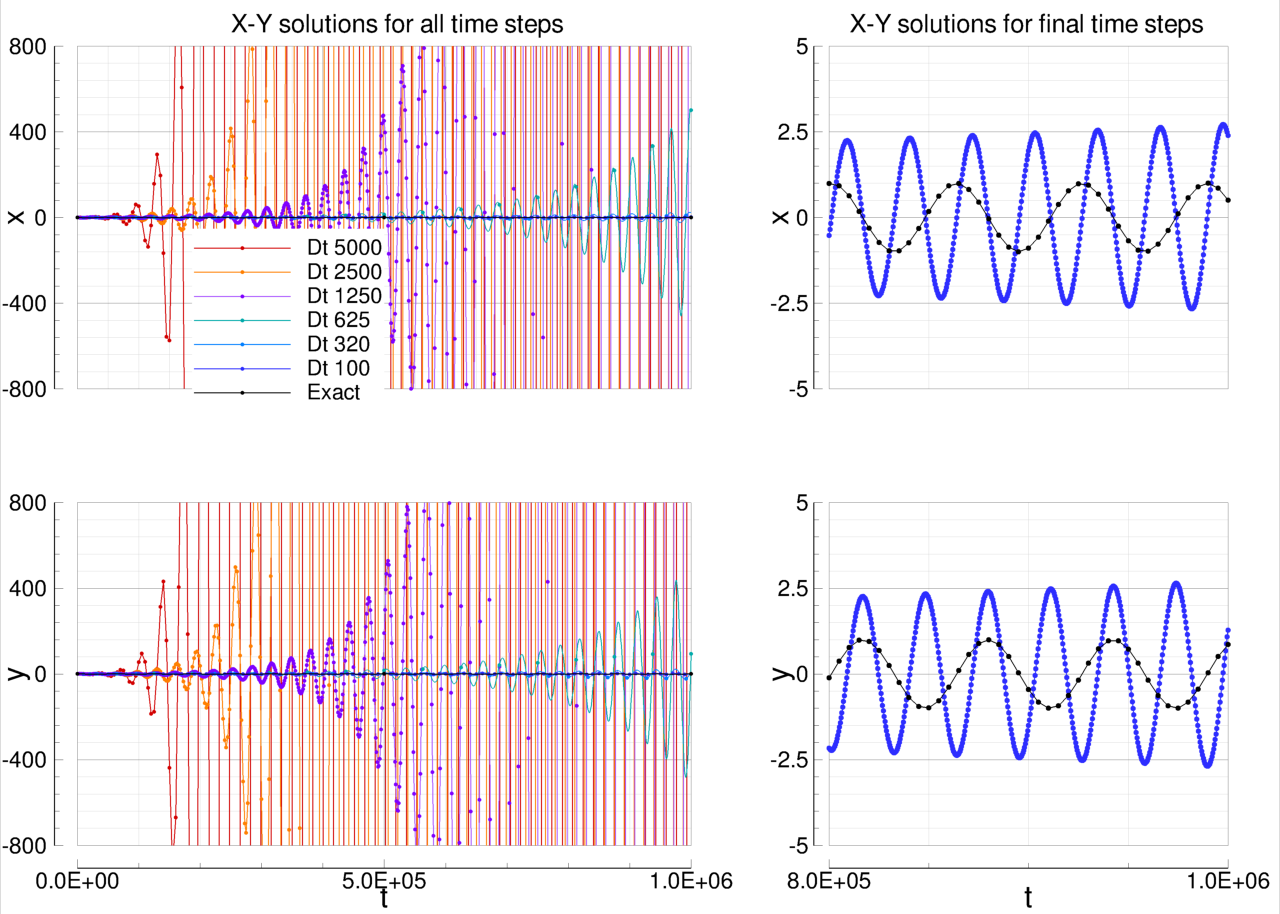
\includegraphics[width=1.00\textwidth]{errors-analysis/oscillation/errors_analysis-oscillation-adams-bashforth-moulton-1.png}
    \caption{1 step}\label{fig:results-oscillation-adams-bashforth-moulton-1}
  \end{subfigure}\quad%
  \begin{subfigure}[b]{0.45\textwidth}
    \centering
    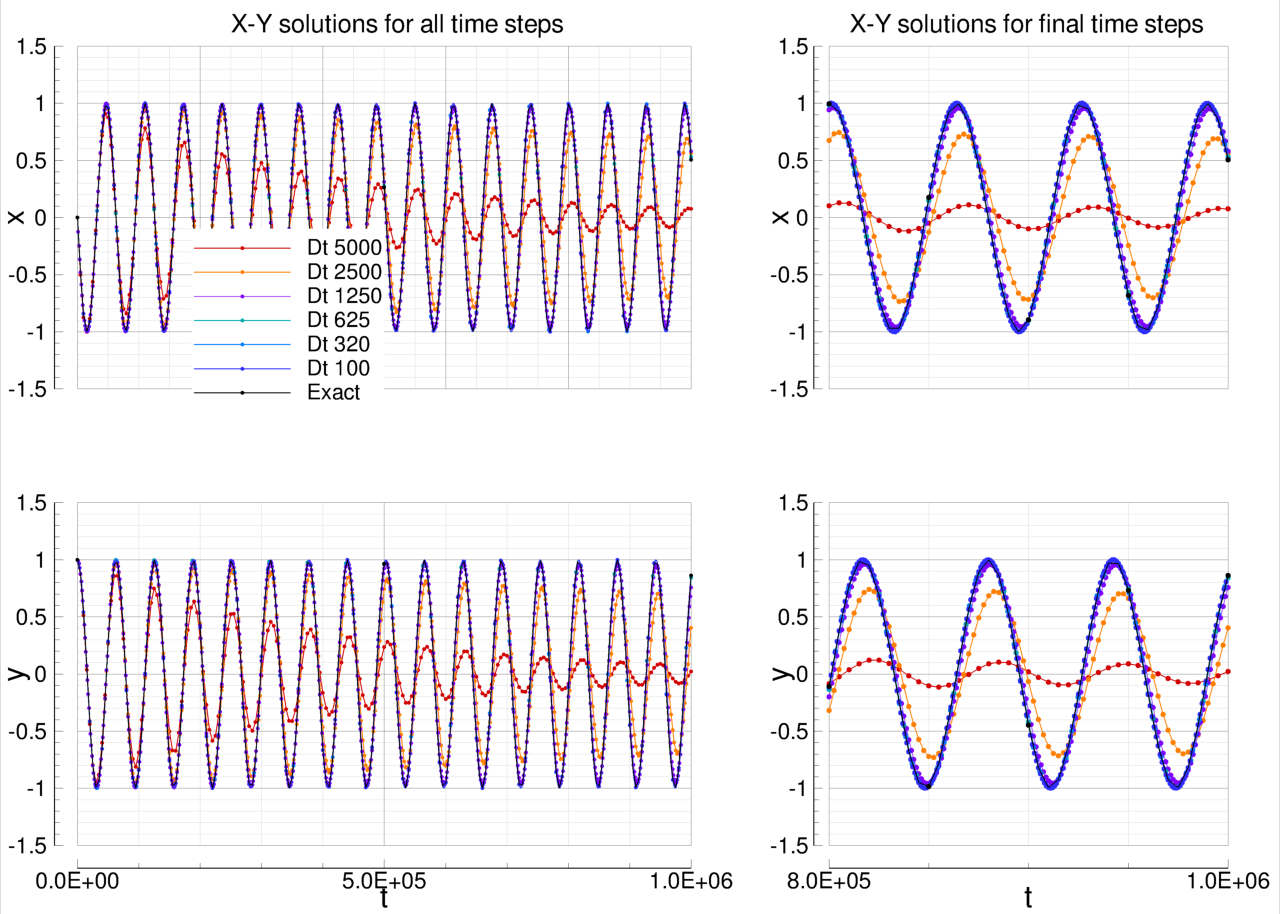
\includegraphics[width=1.00\textwidth]{errors-analysis/oscillation/errors_analysis-oscillation-adams-bashforth-moulton-2.png}
    \caption{2 steps}\label{fig:results-oscillation-adams-bashforth-moulton-2}
  \end{subfigure}\\
  \begin{subfigure}[b]{0.45\textwidth}
    \centering
    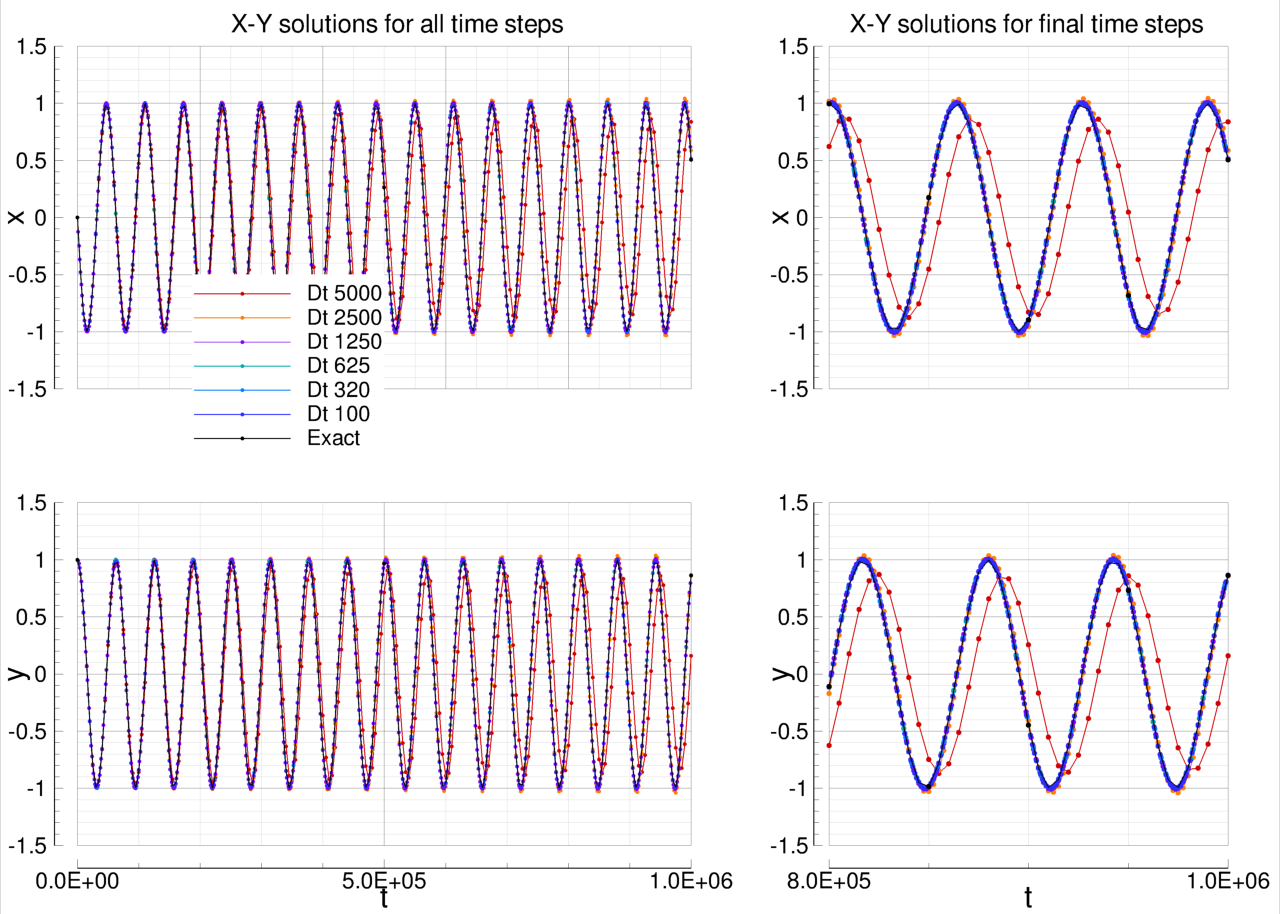
\includegraphics[width=1.00\textwidth]{errors-analysis/oscillation/errors_analysis-oscillation-adams-bashforth-moulton-3.png}
    \caption{3 steps}\label{fig:results-oscillation-adams-bashforth-moulton-3}
  \end{subfigure}\quad%
  \begin{subfigure}[b]{0.45\textwidth}
    \centering
    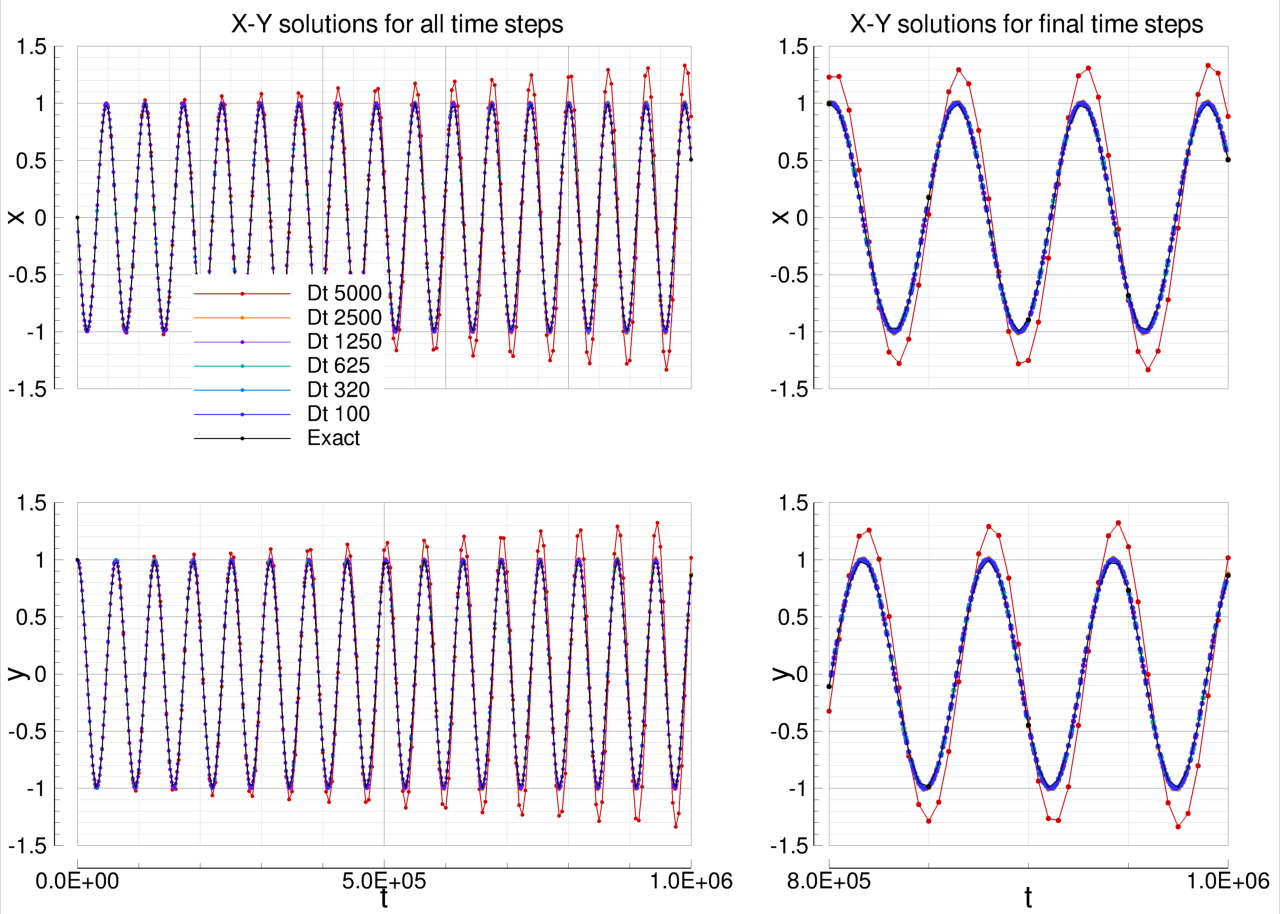
\includegraphics[width=1.00\textwidth]{errors-analysis/oscillation/errors_analysis-oscillation-adams-bashforth-moulton-4.png}
    \caption{4 steps}\label{fig:results-oscillation-adams-bashforth-moulton-4}
  \end{subfigure}
  \caption{Oscillation equations solutions computed by means of Adams-Bashforth-Moulton solvers}\label{fig:results-oscillation-adams-bashforth-moulton}
\end{figure}
\clearpage

